\setcounter{subsection}{3-1}
\subsection{Relations}

% Some useful commands for these exercises
\newcommand\ppt[1]{(x_{#1}, y_{#1})}
\newcommand\peq[1]{y_{#1} - x_{#1}^2}

\exercise{1}{
  Define two points $\ppt{0}$ and $\ppt{1}$ of the plane to be equivalent if $\peq{0} = \peq{1}$.
  Check that this is an equivalence relation and describe the equivalence classes.
}
\sol{
  First we show that this relation, which we shall denote with $\sim$, is an equivalence relation.
  \qproof{
    In what follows, suppose that $\ppt{0}$, $\ppt{1}$, and $\ppt{2}$ are all points in the plane.
    
    (Reflexivity) Of course we have $\peq{0} = \peq{0}$, and hence $\ppt{0} \sim \ppt{0}$.

    (Symmetry) Suppose that $\ppt{0} \sim \ppt{1}$.
    Then we have $\peq{0} = \peq{1}$ so that of course $\peq{1} = \peq{1}$ since numerical equality is symmetric, and so $\ppt{1} \sim \ppt{0}$ as well.

    (Transitivity) Suppose that $\ppt{0} \sim \ppt{1}$ and $\ppt{1} \sim \ppt{2}$.
    Then $\peq{0} = \peq{1}$ and $\peq{1} = \peq{2}$ so that of course $\peq{0} = \peq{2}$ since numerical equality is transitive.
    Therefore $\ppt{0} \sim \ppt{2}$, which shows transitivity.

    This suffices to show that $\sim$ is an equivalence relation as we set out to show.
  }

  Each equivalence class formed by this relation is the parabola $y = x^2$ shifted up or down on the $y$-axis.
  This is easy to see since two points $\ppt{0}$ and $\ppt{1}$ are in the same class if $\peq{0}$ and $\peq{1}$ have the same value, say $c$.
  Then $\peq{0} = c$ so that $y_0 = x_0^2 + c$, which is clearly such a parabola, and similarly $y_1 = x_1^2 + c$.
}

\exercise{2}{
  Let $C$ be a relation on a set $A$.
  If $A_0 \ss A$, define the \boldit{restriction} of $C$ to $A_0$ to be the relation $C \cap (A_0 \times A_0)$.
  We also note that clearly $C_0 \ss C$ as well.
  Show that the restriction of an equivalence relation is an equivalence relation.
}
\sol{
  \qproof{
    Define $C$, $A$, and $A_0$ as above and suppose that $C$ is an equivalence relation.
    Let $C_0 = C \cap (A_0 \times A_0)$ be the restriction of $C$ to $A_0$, noting that this is in fact a relation on $A_0$ since clearly $C_0 \ss A_0 \times A_0$.
    Now we show that $C_0$ satisfies the three properties of an equivalence relation.

    (Reflexivity) Consider any $a \in A_0$ so that of course $(a,a) \in A_0 \times A_0$.
    Since $A_0 \ss A$ we also have that $a \in A$.
    Hence $aCa$ since $C$ is an equivalence relation on $A$ and is therefore reflexive.
    Thus $(a,a) \in C \cap (A_0 \times A_0) = C_0$, which shows that $a C_0 a$ so that $C_0$ is reflexive since $a$ was arbitrary.

    (Symmetry) Suppose that $a,b \in A_0$ and that $aC_0b$.
    Then of course $(b,a) \in A_0 \times A_0$ and $bCa$ since $C_0 \ss C$.
    From this it follows that $(b,a) \in C \cap (A_0 \times A_0) = C_0$ so that $b C_0 a$.
    This of course shows that $C_0$ is symmetric.

    (Transitivity) Now consider $a,b,c \in A_0$ and suppose that both $a C_0 b$ and $b C_0 c$.
    Then we have $aCb$ and $bCc$ since $C_0 \ss C$.
    Since $C$ is an equivalence relation and therefore transitive, it follows that $aCc$, and since also clearly $(a,c) \in A_0 \times A_0$, we have $(a,c) \in C \cap (A_0 \times A_0) = C_0$ so that $a C_0 c$.
    This shows that $C_0$ is transitive.
  }
}

\exercise{3}{
  Here is a ``proof'' that every relation $C$ that is both symmetric and transitive is also reflexive:
  ``Since $C$ is symmetric, $aCb$ implies $bCa$.
  Since $C$ is transitive, $aCb$ and $bCa$ together imply $aCa$, as desired.''
  Find the flaw in this argument.
}
\sol{
  Suppose that $C$ is a relation on the set $A$.
  This argument is perfectly valid for any $a,b \in A$ such that $aCb$, which is to say that we can conclude that $aCa$ in this case (and by the same argument $bCb$).
  However, reflexivity requires $aCa$ to hold for \emph{every} $a \in A$.
  So if there is no $b \in A$ such that $aCb$ then the above argument cannot be applied and we cannot conclude that $aCa$.
  In this case the element $a$ is effectively not involved in the relation at all.

  This is perhaps best illustrated with an example: suppose that $A = \braces{1,2,3,4}$ and
  \gath{
    C = \braces{(1,1), (2,2), (3,3), (1,2), (2,1), (2,3), (3,2), (1,3), (3,1)} \,.
  }
  It is easy to verify that $C$ is both symmetric and transitive on $A$ but it is clearly not reflexive since $(4,4) \notin C$.
  One can also observe how $4$ is not involved in the relation at all and, if it were, it would have to be that $(4,4) \in C$ if $C$ were to remain symmetric and transitive.
}

\exercise{4}{
  Let $f: A \to B$ be a surjective function.
  Let us define a relation on $A$ by setting $a_0 \sim a_1$ if
  \gath{
    f(a_0) = f(a_1) \,.
  }
  \eparts{
  \item Show that this is an equivalence relation.
  \item Let $A^*$ be the set of equivalence classes.
    Show that there is a bijective correspondence of $A^*$ with $B$.
  }
}
\sol{
  (a)
  \qproof{
    We show the three properties necessary for $\sim$ to be an equivalence relation:
    
    (Reflexivity) Consider any $a \in A$ so that of course $f(a) = f(a)$ since $f$ is a function.
    Hence $a \sim a$ so that $\sim$ is reflexive since $a$ was arbitrary.

    (Symmetry) Consider $a,b \in A$ and suppose that $a \sim b$.
    Then by definition $f(a) = f(b)$ so that obviously also $f(b) = f(a)$ since equality is symmetric.
    So of course $b \sim a$, which shows that $\sim$ is symmetric.

    (Transitivity) Consider $a,b,c \in A$ and suppose that $a \sim b$ and $b \sim c$.
    Then by definition $f(a) = f(b)$ and $f(b) = f(c)$ so that of course $f(a) = f(b) = f(c)$, and hence $a \sim c$.
    This shows that $\sim$ is transitive.
  }

  (b)
  \qproof{
    Define the function $g: A^* \to B$ as follows.
    For any equivalence class $C \in A^*$, we know that $C$ is nonempty since $A^*$ is a partition of $A$.
    Hence there is an $a \in C$, so set $g(C) = f(a)$, noting that clearly $g(C) = f(a) \in B$ so that $B$ can be the range of $g$.

    To show that $g$ is injective, consider two equivalence classes $C$ and $D$ where $g(C) = g(D)$.
    Then there are elements $c \in C$ and $d \in D$ where $f(c) = g(C) = g(D) = f(d)$.
    This shows that $c \sim d$ so that they must be in the same equivalence class.
    Thus $d \in C$ since $c \in C$, but also $d \in D$ so that $C$ and $D$ are not disjoint.
    Hence it must be that $C = D$ by Lemma~3.1, which shows that $g$ is injective.

    To show that $g$ is surjective, consider any $b \in B$.
    Since $f$ is surjective, there is an $a \in A$ such that $f(a) = b$.
    Since $A^*$ is a partition, $a$ must belong to an equivalence class $C \in A^*$.
    Then there is an element $c \in C$ such that $g(C) = f(c)$ by the definition of $g$.
    Since $a$ and $c$ are both in the same equivalence class $C$, we have that $a \sim c$ so that $g(C) = f(c) = f(a) = b$.
    This shows that $g$ is surjective since $b \in B$ was arbitrary.

    Therefore we have shown that $g$ is both injective and surjective, and so is a bijection by definition, as desired.
  }
}

\exercise{5}{
  Let $S$ and $S'$ be the following subsets of the plane:
  \ali{
    S &= \braces{\ppt{} \where y = x+1 \text{ and } 0 < x < 2} \,, \\
    S' &= \braces{\ppt{} \where y - x \text{ is an integer}} \,.
  }
  \eparts{
  \item Show that $S'$ is an equivalence relation on the real line and $S' \sps S$.
    Describe the equivalence classes of $S'$.
  \item Show that given any collection of equivalence relations on a set $A$, their intersection is an equivalence relation on $A$.
  \item Describe the equivalence relation $T$ on the real line that is the intersection of all equivalence relations on the real line that contain $S$.
    Describe the equivalence classes of $T$.
  }
}
\sol{
  (a)
  \qproof{
    First note that $S' \ss \reals \times \reals$ and so is a relation on $\reals$.
    We show that $S'$ has the three properties required of an equivalence relation.

    (Reflexivity) Consider any $x \in \reals$ so that clearly $x - x=0$ is an integer.
    Hence $(x,x) \in S'$ by definition.
    This shows that $S'$ is reflexive since $x$ was arbitrary.

    (Symmetry) Suppose that $x,y \in \reals$ and $x S' y$.
    Then $n = y - x$ is an integer so that $x - y = -(y-x) = -n$ is also clearly an integer.
    Therefore $y S' x$ as well, which shows that $S'$ is symmetric.

    (Transitivity) Consider $x,y,z \in \reals$ and suppose that both $x S' y$ and $y S' z$.
    Then $n = y - x$ and $m = z - y$ are both integers.
    We then have
    \gath{
      z - x = z - x + y - y = (z - y) + (y - x) = m + n \,,
    }
    which is clearly an integer since $m$ and $n$ are.
    Hence $x S' z$ so that $S'$ is transitive.

    It is easy to show that $S' \sps S$.
    Consider any $\ppt{} \in S$ so that $0 < x < 2$ and $y = x + 1$.
    Then $y - x = (x + 1) - x = 1$, which is of course an integer.
    Hence $\ppt{} \in S'$, and thus $S' \sps S$ since $\ppt{}$ was arbitrary.
  }

  The equivalence class $C$ containing $x \in \reals$ is the countable set $C = \braces{x + n \where n \in \ints}$.
  While perhaps not immediately obvious, it is almost trivial to show:
  \ali{
    y \in C &\bic \exists n \in \ints (y = x + n) \bic \exists n \in \ints (y - x = n) \\
    &\bic x S' y \bic y S' x \\
    &\bic \text{$y$ is in the equivalence class determined by $x$}
  }
  since $S'$ is symmetric.

  (b)
  \qproof{
    Let $A^*$ be a collection of equivalence relations on $A$ so that we must show that $C = \bigcap_{D \in A^*} D$ is also an equivalence relation on $A$.
    First, suppose that any $\ppt{} \in C$ and consider any $D \in A^*$ so that $\ppt{} \in D$.
    Then also $\ppt{} \in A \times A$ since $D$ is a relation on $A$ so that $D \ss A \times A$.
    This shows that $C \ss A \times A$ since $\ppt{}$ was arbitrary, and so $C$ is a relation on $A$.
    Now we show the three required properties of an equivalence relation:

    (Reflexivity) Consider any $x \in A$ so that $(x,x) \in D$ for every $D \in A^*$ since each $D$ is an equivalence relation and so is reflexive.
    It then follows that $(x,x) \bigcap_{D \in A^*} D = C$, which shows that $C$ is reflexive.

    (Symmetric) Suppose that $\ppt{} \in C$ and consider any $D \in A^*$ so that also $\ppt{} \in D$.
    Then also $(y,x) \in D$ since $D$ is an equivalence relation and so is symmetric.
    Since $D$ was arbitrary, this shows that $(y,x) \in \bigcap_{D \in A^*} D = C$ so that $C$ is symmetric.

    (Transitivity) Suppose that $\ppt{} \in C$ and $(y,z) \in C$.
    For any $D \in A^*$ we then have that both $\ppt{} \in D$ and $(y,z) \in D$.
    It then follows that $(x,z) \in D$ since $D$ is an equivalence relation and so is transitive.
    Since $D$ was arbitrary, we have that $(x,z) \in \bigcap_{D \in A^*} D = C$ so that $C$ is transitive as desired.
  }

  (c)
  First we note that $S$ itself is \emph{not} an equivalence relation on $\reals$ since it is not reflexive.
  In fact $(x,x) \notin S$ for any $x \in \reals$ since it is never true that $x = x+1$.
  Now define the following subsets of the plane:
  \ali{
    S_1 &= \braces{\ppt{} \where y = x} &
    S_4 &= \braces{\ppt{} \where y = x + 2 \text{ and } 0 < x < 1} \\
    S_2 &= S = \braces{\ppt{} \where y = x + 1 \text{ and } 0 < x < 2} &
    S_5 &= \braces{\ppt{} \where y = x - 2 \text{ and } 2 < x < 3} \,. \\
    S_3 &= \braces{\ppt{} \where y = x - 1 \text{ and } 1 < x < 3}
  }
  We then claim that the intersection we seek is $T = \bigcup_{i \in \intsfin{5}} S_i$.
  An illustration of this set in the plane is shown below:
  \begin{center}
    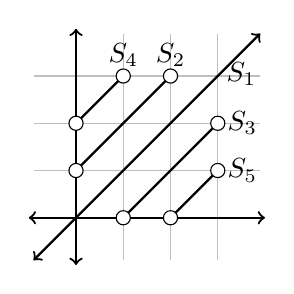
\begin{tikzpicture}[scale=0.6]
      % Open line
      \newcommand\oline[2]{
        \draw[thick,-] (#1) -- (#2);
        \filldraw[fill=white] (#1) circle (0.15);
        \filldraw[fill=white] (#2) circle (0.15);
      }
      % Coordinate grid
      \draw[step=1cm,black!25!white,thin] (-0.9,-0.9) grid (3.9,3.9);

      % Axes
      \draw[thick,<->] (-1,0) -- (4,0);
      \draw[thick,<->] (0,-1) -- (0,4);

      % Subsets
      \draw[thick,<->] (-0.9,-0.9) -- (3.9,3.9);
      \node [below] at (3.5,3.5) {$S_1$};
      \oline{0,1}{2,3}
      \node [above] at (2,3) {$S_2$};
      \oline{1,0}{3,2}
      \node [right] at (3,2) {$S_3$};
      \oline{0,2}{1,3}
      \node [above] at (1,3) {$S_4$};
      \oline{2,0}{3,1}
      \node [right] at (3,1) {$S_5$};
    \end{tikzpicture}
  \end{center}
  \qproof{
    Let $S^*$ denote the collection of all equivalence relations on $\reals$ that contain $S$ so that we must show that $T = \bigcap_{R \in S^*} R$.

    $(\ss)$ Consider any $\ppt{} \in T$ and any $R \in S^*$ so that $R$ is an equivalence relation on $\reals$ that contains $S$.
    We then have the following cases:

    Case: $\ppt{} \in S_1$.
    Then of course $y = x$ so that $\ppt{} = (x,x) \in R$ since it is an equivalence relation and thus reflexive.

    Case: $\ppt{} \in S_2 = S$.
    Then of course $\ppt{} \in R$ since $R$ contains $S$.

    Case: $\ppt{} \in S_3$.
    Then we have that $y = x - 1$ with $1 < x < 3$, from which it follows that $x = y + 1$ and $0 < y = x-1 < 2$.
    Therefore $(y,x) \in S$ so that $(y,x) \in R$ since $R$ contains $S$.
    We then have that $\ppt{} \in R$ as well since $R$ is an equivalence relation and therefore symmetric.

    Case: $\ppt{} \in S_4$.
    Then $y = x+2$ with $0 < x < 1$.
    Let $z = x+1$ so that $(x,z) \in S = S_4$ since we also have $0 < x < 1 < 2$.
    We then know that $(x,z) \in R$ since $R$ contains $S$.
    We also then have that $y = x+2 = (x+1)+1 = z+1$ with $0 < 1 < z = x+1 < 2$ since $0 < x < 1$.
    Thus $(z,y) \in S = S_4$ so that also $(z,y) \in R$.
    Since $R$ is an equivalence relation and therefore transitive, we have that $\ppt{} \in R$ as well.

    Case: $\ppt{} \in S_5$.
    Then we have $y = x-2$ and $2 < x < 3$.
    It then follows that $x = y+2$ and $0 < y = x-2 < 1$ so that $(y,x) \in S_4$.
    Then of course $(y,x) \in R$ by the previous case so that also $\ppt{} \in R$ since $R$ is an equivalence relation and therefore symmetric.

    Thus in every case $\ppt{} \in R$ so that also $\ppt{} \in \bigcap_{R \in S^*} R$ since $R$ was arbitrary.
    It then follows that $T \ss \bigcap_{R \in S^*} R$ since $\ppt{}$ was arbitrary.

    $(\sps)$ All we really need to show is that $T$ is an equivalence relation on $\reals$ that contains $S$.
    From this it follows that $T \in S^*$ so that of course $T \sps \bigcap_{R \in S^*} R$.
    First we note that clearly $T \ss \reals^2$ so that it is a relation on $\reals$.
    Also clearly it contains $S$ since $S = S_2 \ss T$.
    Now we show that it has the three properties that an equivalence relation require.

    (Reflexivity) For any $x \in \reals$ clearly $(x,x) \in S_1 \ss T$ so that $T$ is reflexive.

    (Symmetry) Suppose that $xTy$ so that $\ppt{} \in T$.
    We then have the following cases:

    Case: $\ppt{} \in S_1$.
    Then of course $y = x$ so $(y,x) = (x,x) = \ppt{} \in S_1 \ss T$.

    Case: $\ppt{} \in S_2 = S$.
    Then $y = x+1$ and $0<x<2$ so that $x = y-1$ and $1 < y=x+1 < 3$.
    Hence $(y,x) \in S_3 \ss T$.

    Case: $\ppt{} \in S_3$.
    Then we have that $y = x - 1$ with $1 < x < 3$, from which it follows that $x = y + 1$ and $0 < y = x-1 < 2$.
    Therefore $(y,x) \in S = S_2 \ss T$.

    Case: $\ppt{} \in S_4$.
    Then $y = x+2$ with $0 < x < 1$ so that $x = y-2$ and $2 < y=x+2 < 3$.
    Hence $(y,x) \in S_5 \ss T$.

    Case: $\ppt{} \in S_5$.
    Then we have $y = x-2$ and $2 < x < 3$ so that $x = y+2$ and $0 < y=x-2 < 1$.
    Hence $(y,x) \in S_4 \ss T$.

    So in all cases $(y,x) \in T$, which shows that $T$ is symmetric.

    (Transitivity) Now suppose that $xTy$ and $yTz$.
    If $x = y$ then of course we have $(x,z) = (y,z) \in T$.
    Similarly if $y = z$ then $(x,z) = \ppt{} \in T$.
    So assume that $x \neq y$ and $y \neq z$ so that it can neither be that $\ppt{} \in S_1$ nor $(y,z) \in S_1$.
    Thus there are four sets (i.e. $S_i$ where $i \in \braces{2,3,4,5}$) that $\ppt{}$ and $(y,z)$ can be in, which results in sixteen different possibilities, though not all are possible:

    Case: $\ppt{} \in S_2$.
    Then $y=x+1$ and $0 < x < 2$ so that $1 < y = x+1 < 3$.
    \begin{indpar}
      Case: $(y,z) \in S_2$.
      Then also $z=y+1$ and $0 < y < 2$ so that $z = y+1 = (x+1)+1 = x+2$ and $y = x+1 < 2$ means that $x < 1$.
      Hence $z = x+2$ and $0 < x < 1$ so that $(x,z) \in S_4 \ss T$.

      Case: $(y,z) \in S_3$.
      Then $z = y-1$ and $1 < y < 3$ so that $z = y-1 = (x+1)-1 = x$, and hence $(x,z) = (x,x) \in S_1 \ss T$.

      Case: $(y,z) \in S_4$.
      This case is not possible because $1 < y < 3$ so that it cannot be that $0 < y < 1$ and hence $(y,z)$ cannot be in $S_4$.

      Case: $(y,z) \in S_5$.
      Then $z = y-2$ and $2 < y < 3$ so that $z = y-2 = (x+1)-2 = x-1$ and $2 < y = x+1 < 3$ means that $1 < x < 2 < 3$.
      Hence $z=x-1$ and $1 < x < 3$ so that $(x,z) \in S_3 \ss T$.
    \end{indpar}

    Case: $\ppt{} \in S_3$.
    Then $y=x-1$ and $1 < x < 3$ so that $0 < y = x-1 < 2$.
    \begin{indpar}
      Case: $(y,z) \in S_2$.
      Then $z = y+1$ and $0 < y < 2$ so that $z = y+1 = (x-1)+1 = x$ and hence $(x,z) = (x,x) \in S_1 \ss T$.

      Case: $(y,z) \in S_3$.
      Then $z = y-1$ and $1 < y < 3$ so that $z = y-1 = (x-1)-1 = x-2$ and $1 < y = x-1$ and hence $2 < x$.
      Therefore $z = x-2$ and $2 < x < 3$ so that $(x,z) \in S_5 \ss T$.

      Case: $(y,z) \in S_4$.
      Then $z=y+2$ and $0 < y < 1$ so that $z = y+2 = (x-1)+2 = x+1$ and $y = x-1 < 1$ and hence $x < 2$.
      Thus $z = x+1$ and $0 < 1 < x < 2$ so that $(x,z) \in S_2 \ss T$.

      Case: $(y,z) \in S_5$.
      This is case is not possible because $y < 2$ so that it cannot be that $2 < y < 3$, and hence $(y,z)$ cannot be in $S_5$.
    \end{indpar}

    Case: $\ppt{} \in S_4$.
    Then $y=x+2$ and $0 < x < 1$ so that $2 < y = x+2 < 3$.
    \begin{indpar}
      Case: $(y,z) \in S_2$.
      This case is also impossible because $2 < y$  so that it cannot be that $0 < y < 2$, and hence $(y,z)$ cannot be in $S_2$.

      Case: $(y,z) \in S_3$.
      Then $z = y-1$ and $1 < y < 3$ so that $z = y-1 = (x+2)-1 = x+1$ and $y = x+2 < 3$ so that $x < 1 < 2$.
      Thus $z = x+1$ and $0 < x < 2$ so that $(x,z) \in S_2 \ss T$.

      Case: $(y,z) \in S_4$.
      This case is not possible because again $2 < y$ so that it cannot be that $0 < y < 1$, and hence $(y,z)$ cannot be in $S_4$.

      Case: $(y,z) \in S_5$.
      Then $z=y-2$ and $0 < y <1$ so that $z=y-2=(x+2)-2=x$ and hence $(x,z) = (x,x) \in S_1 \ss T$.
    \end{indpar}

    Case: $\ppt{} \in S_5$.
    Then $y=x-2$ and $2 < x < 3$ so that $0 < y=x-2 < 1$.
    \begin{indpar}
      Case: $(y,z) \in S_2$.
      Then $z = y+1$ and $0 < y < 2$ so that $z = y+1 = (x-2) + 1 = x-1$ and $0 < y = x-2$ so that $1 < 2 < x$.
      Therefore $z=x-1$ and $1 < x < 3$ so that $(x,z) \in S_3 \ss T$.

      Case: $(y,z) \in S_3$.
      This case is not possible because $y < 1$ so that it cannot be that $1 < y < 3$, and hence $(y,z)$ cannot be in $S_3$.

      Case: $(y,z) \in S_4$.
      Then $z = y+2$ and $0 < y < 1$ so that $z = y+2 = (x-2)+2$ and hence $(z,x) = (x,x) \in S_1 \ss T$.

      Case: $(y,z) \in S_5$.
      This case is also not possible because again $y < 1$ so that it cannot be that $2 < y < 3$, and hence $(y,z)$ cannot be in $S_5$.
    \end{indpar}

    Thus in every case that is actually possible we have that $(x,z) \in T$, which shows that $T$ is transitive.

    Therefore $T$ is an equivalence relation that contains $S$ so that $T \sps \bigcap_{R \in S^*} R$ as discussed above, which of course completes the proof that $T = \bigcap_{R \in S^*} R$.
  }

  As far as the equivalence classes formed by $T$ are concerned, refer to the illustration above.
  Consider the equivalence class $C$ contains $x \in \reals$.
  If $x \leq 0$ or $x \geq 3$ then $C = \braces{x}$ because there is no other $y$ for which $yTx$ except $y=x$.
  So suppose that $0 < x < 3$.
  If $x$ is an integer so that $x = 1$ or $x = 2$, then $C = \braces{1,2}$.
  If $x$ is not an integer, then $C$ always has three elements.
  We have that
  \gath{
    C = \begin{cases}
      \braces{x, x+1, x+2} & 0 < x < 1 \\
      \braces{x-1, x, x+1} & 1 < x < 2 \\
      \braces{x-2, x-1, x} & 2 < x < 3
    \end{cases} \,.
  }
  These facts can be deduced by examining where the vertical line intersecting the $x$-axis at $x$ intersects the graph of $T$.
}

\exercise{6}{
  Define a relation on the plane by setting
  \gath{
    \ppt{0} < \ppt{1}
  }
  if either $y_0 - x_0^2 < y_1 - x_1^2$ or $y_0 - x_0^2 = y_1 - x_1^2$ and $x_0 < x_1$.
  Show that this is an order relation on the plane, and describe it geometrically.
}
\sol{
  First we show that $<$ is an order relation on the plane.
  \qproof{
    As clearly $<$ is a relation on the plane, we need only show that it has the three required properties of an order relation:

    (Comparability) Consider distinct $\ppt{0}$ and $\ppt{1}$ in the plane so that either $x_0 \neq x_1$ or $y_0 \neq y_1$.
    Obviously if $\peq{0} < \peq{1}$ (or $\peq{1} < \peq{0}$) then of course $\ppt{0} < \ppt{1}$ (or $\ppt{1} < \ppt{0}$) so we are done.
    So assume that $\peq{0} = \peq{1}$.
    It it were the case that $x_0 = x_1$ it would have to be that $y_0 \neq y_1$, but we would have
    \gath{
      \peq{0} = \peq{1} = y_1 - x_0^2 \\
      y_0 = y_1 \,,
    }
    which is a contradiction.
    So it must be that $x_0 \neq x_1$.
    So either $x_0 < x_1$ and so $\ppt{0} < \ppt{0}$ or $x_1 < x_0$ and so $\ppt{1} < \ppt{0}$.
    This shows that $<$ is comparable in the plane.

    (Nonreflexivity) Consider $\ppt{}$ in the plane so that obviously $\peq{} = \peq{}$.
    As we also have that $x = x$, it is not the case that $x < x$ so that it is not true that $\ppt{} < \ppt{}$.

    (Transitivity) Suppose that $\ppt{0} < \ppt{1}$ and $\ppt{1} < \ppt{2}$.
    We then have the following:

    Case: $\peq{0} < \peq{1}$.
    \begin{indpar}
      Case:  $\peq{1} < \peq{2}$.
      Then of course $\peq{0} < \peq{1} < \peq{2}$ so that $\ppt{0} < \ppt{2}$.

      Case: $\peq{1} = \peq{2}$ and $x_1 < x_2$.
      Then we have $\peq{0} < \peq{1} = \peq{2}$ so that again $\ppt{0} < \ppt{2}$.
    \end{indpar}

    Case: $\peq{0} = \peq{1}$ and $x_0 < x_1$.
    \begin{indpar}
      Case: $\peq{1} < \peq{2}$.
      Then $\peq{0} = \peq{1} < \peq{2}$ so that $\ppt{0} < \ppt{2}$.

      Case: $\peq{1} = \peq{2}$ and $x_1 < x_2$.
      Then $\peq{0} = \peq{1} = \peq{2}$ and $x_0 < x_1 < x_2$ so that $\ppt{0} < \ppt{2}$.
    \end{indpar}

    Thus in all cases $\ppt{0} < \ppt{2}$, which shows that $<$ is transitive in the plane.
  }

  Geometrically, we refer back to Exercise~3.1 and consider a parabola $y = x^2$ shifted up or down on the $y$-axis be some amount $c$.
  Then $y = x^2 + c$ so that $\peq{} = c$, and hence every $\ppt{}$ point on the parabola has the same value for $\peq{}$, namely $c$.
  Therefore if two distinct points $\ppt{0}$ and $\ppt{1}$ lie on the different parabolas then $\peq{0}$ and $\peq{1}$ will have different values, say $c$ and $d$, respectively.
  Then clearly if $\ppt{1}$ is on a higher parabola on the $y$-axis then $c < d$ so that $\peq{0} = c < d = \peq{1}$ so that $\ppt{0} < \ppt{1}$ in our order.
  If the points lie on the same parabola then $\peq{0} = \peq{1}$ and whichever points is further to the right will be larger in our order since then, for example, $x_0 < x_1$ so that $\ppt{0} < \ppt{1}$.
}

\exercise{7}{
  Show that the restriction of an order relation is an order relation.
}
\sol{
  \qproof{
    Suppose that $A$ is a set with order relation $<$.
    Also let $A_0$ be a subset of $A$ so that $\prec = < \cap (A_0 \times A_0)$ is the restriction of $<$ to $A_0$.
    Clearly $\prec \ss A_0 \times A_0$ so that it s a relation on $A_0$.
    So we must show that $\prec$ satisfies the three properties of an order relation:

    (Comparability) Consider any $x,y \in A_0$ so that also $x,y \in A$ since $A_0 \ss A$.
    Then $x$ and $y$ are comparable in $<$ since it is an order.
    So, without loss of generality, we can assume that $x < y$ and so $(x,y) \in <$.
    Since clearly also $(x,y) \in A_0 \times A_0$, it follows that $(x,y) \in < \cap (A_0 \times A_0) = \prec$ and hence $x \prec y$.
    This shows that $x$ and $y$ are comparable in $\prec$.

    (Nonreflexivity) Suppose that $x \in A_0$ so that also $x \in A$ since $A_0 \ss A$.
    Then it cannot be true that $x < x$ since $A$ is an order and so is nonreflexive.
    Thus $(x,x) \notin <$ so that also $(x,x) \notin < \cap (A_0 \times A_0) = \prec$.
    Hence it is not true that $x \prec x$ so that $\prec$ is also nonreflexive since $x$ was arbitrary.

    (Transitivity) Suppose that $x \prec y$ and $y \prec z$.
    Then of course $(x,y) \in A_0 \times A_0$ and $(x,y) \in <$, and similarly $(y,z) \in A_0 \times A_0$ and $(y,z) \in <$.
    Hence $x < y$ and $y < z$ so that $x < z$ since $<$ is an order and therefore transitive.
    Thus $(x,z) \in <$ so that $(x,z) \in < \cap (A_0 \times A_0) = \prec$ since clearly $(x,z) \in A_0 \times A_0$.
    So then $x \prec z$, which shows that $\prec$ is transitive.
  }
}

\exercise{8}{
  Check that the relation defined in Example~7 is an order relation.
}
\sol{
  Recall that Example~7 is the relation on $C$ on the real line such that $xCy$ if $x^2 < y^2$ or $x^2 = y^2$ and $x < y$.
  \qproof{
    We show that this satisfies the three properties of an order:

    (Comparability) Suppose that $x$ and $y$ are distinct real numbers.
    If $x^2 < y^2$ (or $y^2 < x^2$) then of course $xCy$ (or $yCx$) so we are done.
    So assume that $x^2 = y^2$.
    Since we know that $x \neq y$, it has to be that $y = -x$ so that still $x^2 = y^2$.
    This also implies that $x,y \neq 0$ since otherwise we would have $0 = y = -x = 0 = x$.
    If $x > 0$ then we have $y = -x < 0 < x$.
    If $x < 0$ then we have $x < 0 < -x = y$.
    Hence either way $x^2 = y^2$ but $x < y$ (or $y < x$) so that $xC$ (or $yCx$).
    This shows that $x$ and $y$ are comparable in $C$.

    (Nonreflexivity) Suppose that $x \in \reals$ so that of course $x^2 = x^2$.
    However clearly it is not the case that $x < x$ so that it cannot be that $xCx$ in this relation.

    (Transitivity) Suppose that $xCy$ and $yCz$.
    We then have the following cases:

    Case: $x^2 < y^2$.
    \begin{indpar}
      Case: $y^2 < z^2$.
      Then clearly $x^2 < y^2 < z^2$ so that $xCz$.

      Case: $y^2 = z^2$ and $y < z$.
      Then $x^2 < y^2 = z^2$ so that again $xCz$.
    \end{indpar}

    Case: $x^2 = y^2$ and $x < y$.
    \begin{indpar}
      Case: $y^2 < z^2$.
      Then we have $x^2 = y^2 < z^2$ so that $xCz$.
      
      Case: $y^2 = z^2$ and $y < z$.
      Then $x^2 = y^ = z^2$ and $x < y < z$ so that again $xCz$.
    \end{indpar}

    Hence in all cases $xCz$ so that $C$ is also transitive.
  }

  We note that this order relation differs from the normal order on $\reals$.
  For example if $x = -2$ and $y = 1$ then clearly $x < y$ in the normal order.
  However, we have that $y^2 = 1^2 = 1 < 4 = (-2)^2 = x^2$ so that $yCx$.
}
